%======================================================================
\subsection{BW-SIM-07 P1 --- Built, 1 Nov: the window shell}\label{sec:sim07-shell-built}
%======================================================================

The first phase of the Simulation workspace (answers W1--W3, W6, W9 of \S\ref{sec:sim07-plan}) is in: the window, the
step ribbon, the run panes and the look. The Model Builder tree and the Settings forms that go in the two left docks
are the next agent's (\file{bruceworx\_sim\_model.py}); until then each dock shows the active study's name and a
placeholder line. All Python: \file{bruceworx\_sim\_workspace.py} (the shell),
\file{bruceworx\_sim\_events.py} (run events), the ribbon in \file{bruceworx\_workspaces.py} and
\file{workspaces.json}.

\begin{figure}[!htbp]
\centering
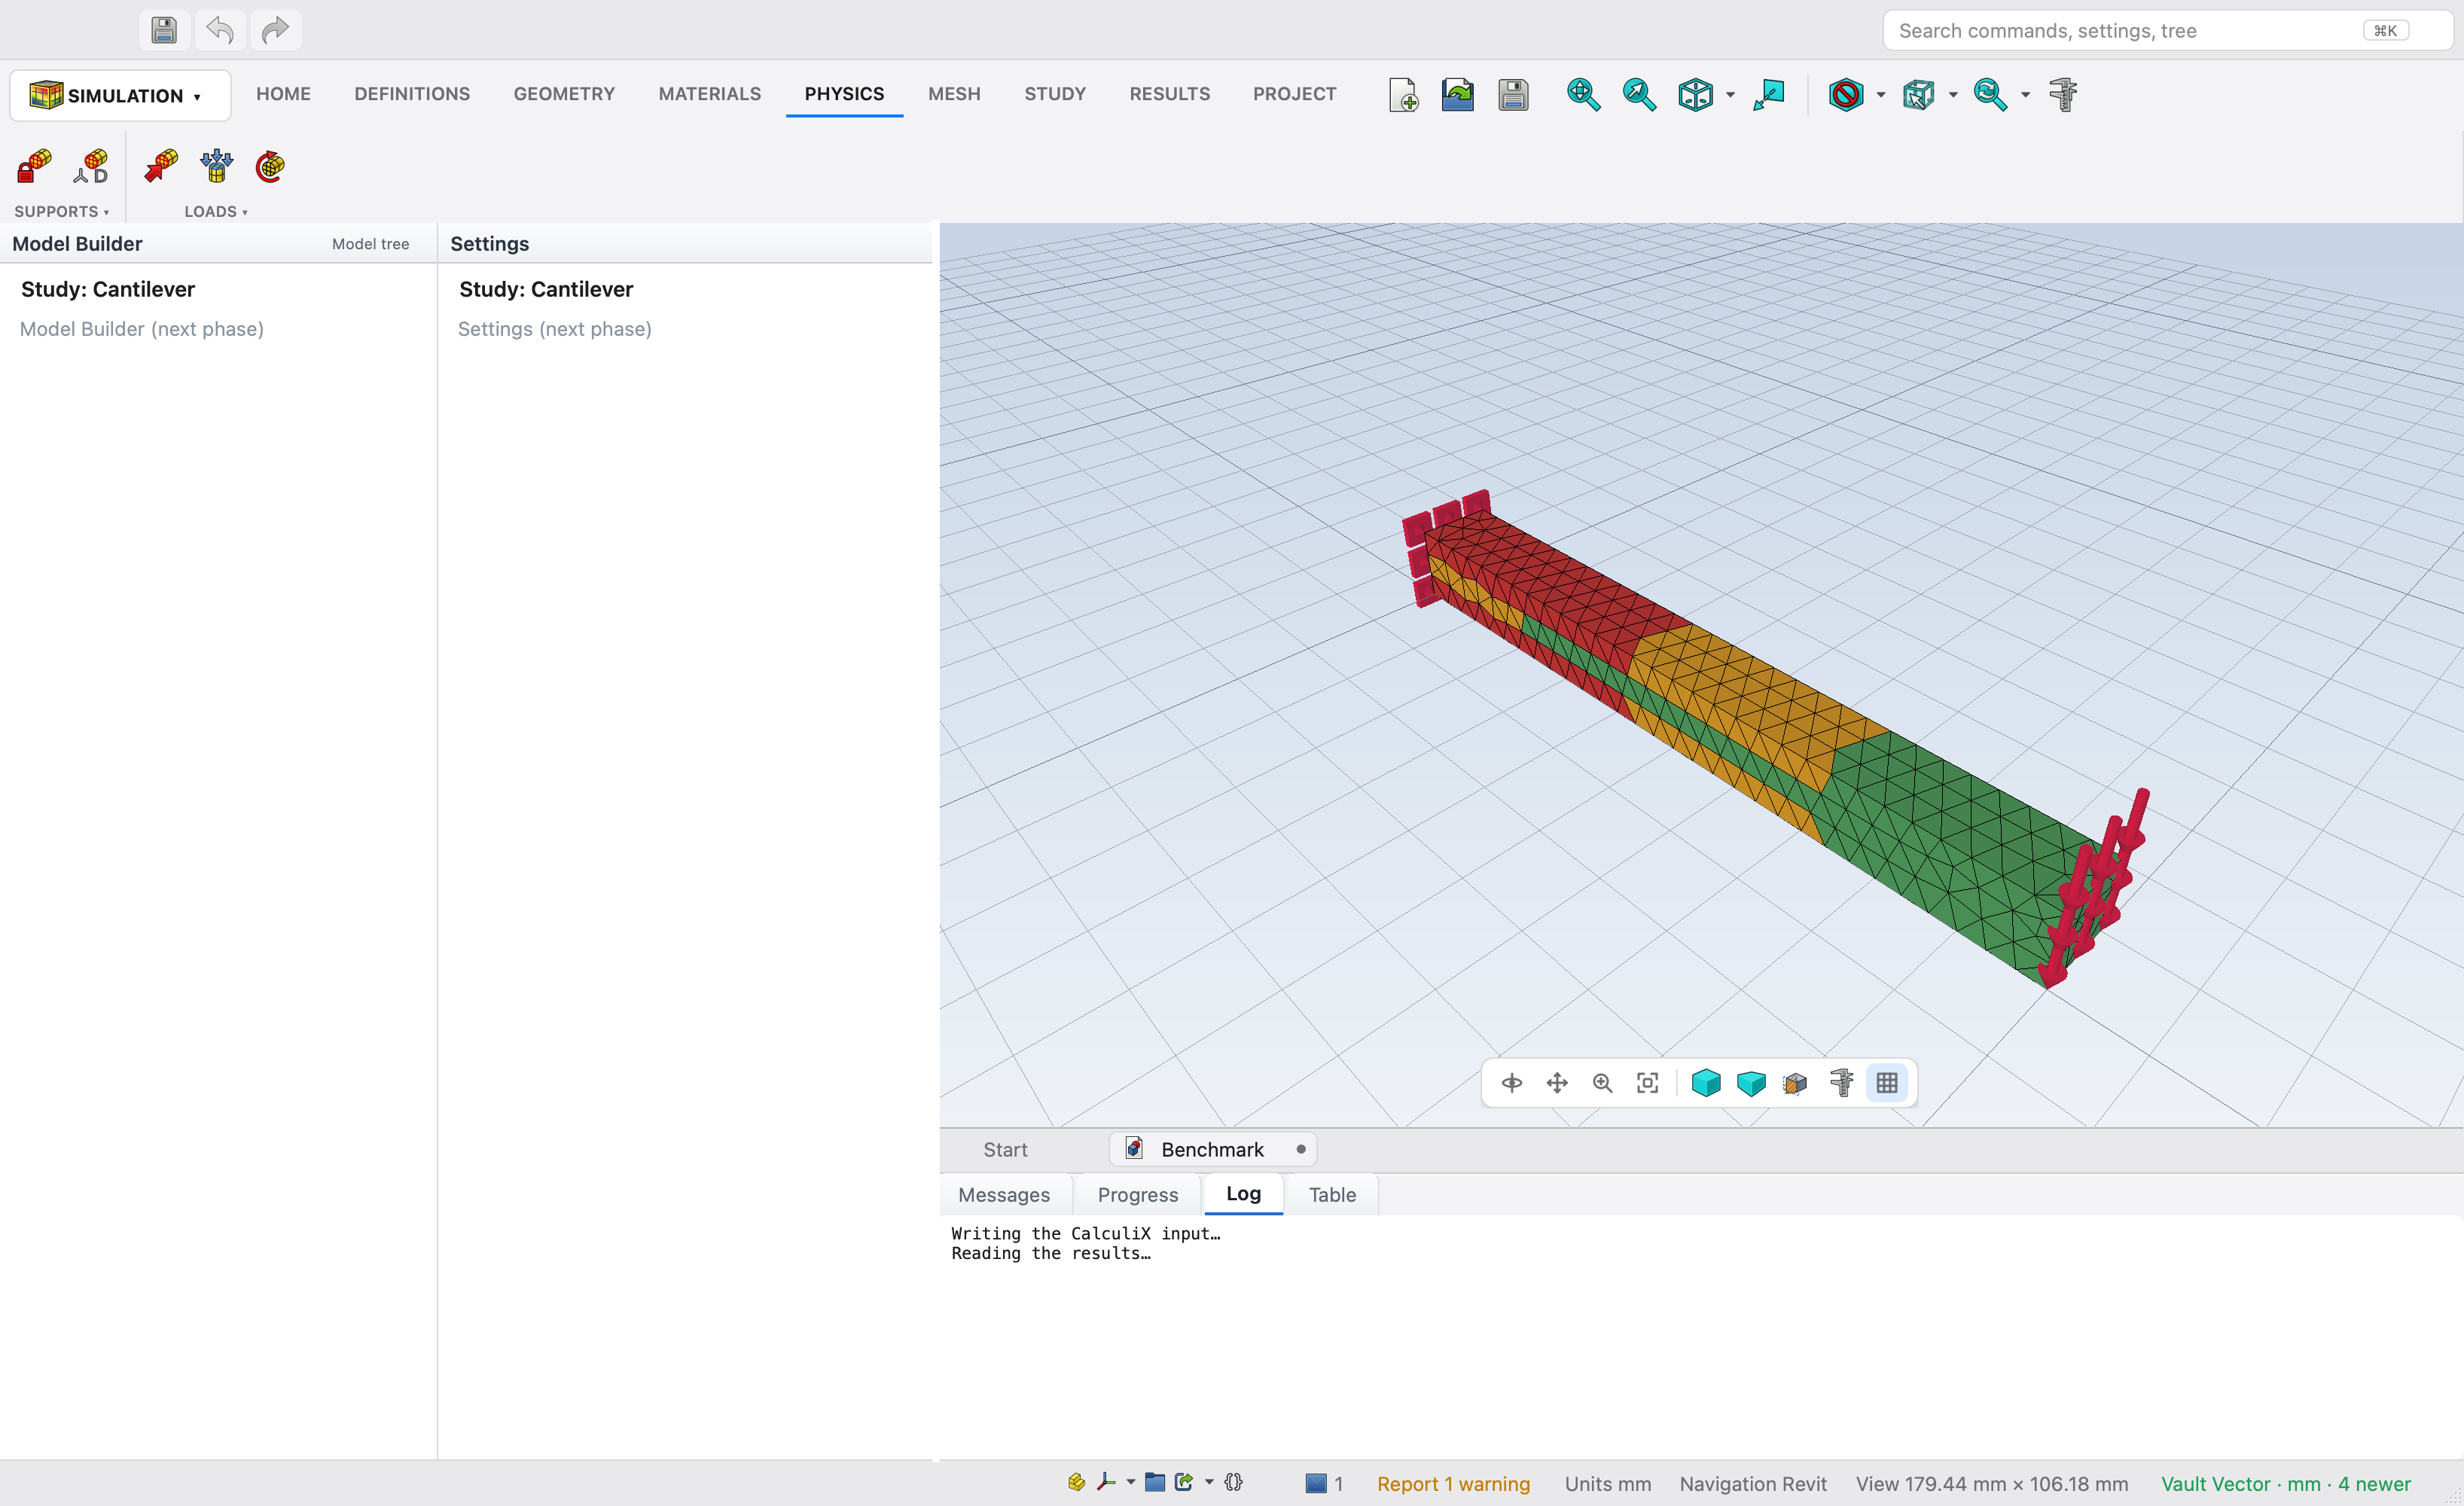
\includegraphics[width=\linewidth]{fig/simui_p1_shell.png}
\caption{The shell after a static solve of the cantilever (off-screen render of the real window): Model Builder and
Settings docks on the left with their placeholders, the 3D view with the light-blue gradient and the axis triad,
Messages under it, and the step ribbon with a Physics tab showing only the structural groups.}
\label{fig:sim07-shell}
\end{figure}

\paragraph{What you can do now.}
\begin{itemize}[nosep]
  \item \textbf{The layout.} Switching to Simulation adds three docks and puts away FreeCAD's model tree and the right
        panel with its floating task view (FreeCAD's auto hide, so a command's task panel still slides in). Model
        Builder (290\,px) and Settings (330\,px) sit left of the 3D view; the bottom dock (190\,px) is under the 3D
        view only, not under the tree. Below 1500\,px window width the two stack in one column. A \emph{Model tree}
        button in the Model Builder header shows and puts away the FreeCAD tree. Switching to any other workspace
        removes the docks and restores the panels, the background and the triad.
  \item \textbf{Messages, Progress, Log, Table.} Messages: one row per message, with a level icon, the time and the
        text; pre-check findings from the study panel and the airflow panel arrive here, and an error brings the
        tab forward. Progress: one row per stage with a bar (busy until a fraction is known, green when done, red
        when it failed) and its time, counting up while it runs. Log: the solver's own lines in a monospace pane.
        Table: empty for now.
  \item \textbf{What feeds them.} Meshing (\emph{Mesh}), the CalculiX input (\emph{Write input}), \emph{Solve} (in
        the panel's QProcess the output is merged and read line by line, so the window stays live as before) and
        \emph{Read results}; for OpenFOAM the stages of the case's \code{log.run}, the solver's own
        \code{log.<stage>} lines, the iteration as a progress fraction, and the latest residuals.
  \item \textbf{The step ribbon.} Nine tabs: Home, Definitions, Geometry, Materials, Physics, Mesh, Study, Results,
        Project. Each group may name the study types it is for; the bar shows the tabs and groups of the active
        study and follows it (checked every 0.6\,s while the workspace is up). A static study shows Fixed,
        Displacement, Force, Pressure, Spin and the stress results; a prop-wash or external-flow study has no Materials or Mesh
        tab and shows Flow setup, Show flow and ParaView; thermal studies show the four thermal loads and the
        temperature results; modal and buckling studies show the supports and the mode shapes. With no study only New
        Study and the placeholders show. Definitions, Geometry and Project hold placeholder commands that say which
        phase brings them.
  \item \textbf{The look.} One stylesheet (\code{stylesheet()}) from the mockup's tokens: 21\,px tree rows, 22\,px
        fields, gradient section and pane headers, accent \code{\#1f6fd1}, applied to the three docks only. The 3D
        view gets the gradient \code{\#c6d4e6} to \code{\#eef2f7} and the axis triad; the preferences and each view's
        own triad setting come back on leaving.
\end{itemize}

\paragraph{For the next agent.} \code{model\_builder\_host()}, \code{settings\_host()} and \code{messages\_pane()}
return the widgets (None headless); \code{clear\_host(host)} removes the placeholders; \code{section(title)} makes a
collapsible Settings section with the gradient header; \code{active\_kind()} and \code{active\_study()} give the study.
Events: \code{bruceworx\_sim\_events.subscribe(listener, replay=True)}, and a node key on a message is kept in the
item's data (\code{Qt.UserRole}) for click-to-select.

\paragraph{Decided while building.}
\begin{itemize}[nosep]
  \item \textbf{Groups are filtered, commands are not.} A group carries \code{"studies": [...]} (a type or a family:
        structural, solid, thermal, airflow), and the bar hides the group's toolbar, rather than greying single
        commands inside a toolbar. This extends the existing tab and toolbar mechanism: no second ribbon.
  \item \textbf{Events are harmless.} Emitting with nobody listening does nothing; a listener that raises is dropped
        with a console warning; the pane receives them through a queued signal, so a runner on another thread cannot
        touch the widgets.
  \item \textbf{Overlays by auto hide, not by closing.} The model tree and the task view keep their state and come
        back exactly as they were.
  \item \textbf{FreeCAD's signal comes early.} \code{workbenchActivated} fires before the workbench is the active one;
        the shell looks a tick later, as the workspace bar does.
\end{itemize}

\paragraph{Tests.} \file{TestBruceWorxSimWorkspace} (21): events (no listener, payloads, a broken listener, the
stage context, history replay, the OpenFOAM feed on a fake case), the ribbon for static, thermal, modal, prop-wash and
no study, and in the GUI: docks appear and disappear, the model tree hidden and restored, stacked below 1500\,px and
columns above, the gradient and triad restored, fake events reaching the three panes, one real static solve of the
cantilever (stages Write input, Solve, Read results, the log and the messages), and the bar's tabs and visible groups
following the study type. \file{TestBruceWorxWorkspaces} and the ribbon test of \file{TestBruceWorxSimulation} were
changed to the nine tabs.

\paragraph{Open questions for you.}
\begin{enumerate}[nosep]
  \item \textbf{Hover at the edge.} The put-away panels still slide in when the mouse touches the window's right
        edge (FreeCAD's auto hide). Hide the right panel completely in this workspace?
  \item \textbf{Airflow commands} are three small ones (Flow setup, Show flow, ParaView) that open the existing panel.
        Is that enough for the Physics and Results tabs until the airflow nodes of P2--P3?
  \item \textbf{A study with no study type tabs.} With no study the Study and Results tabs show a Run and a Report
        group that are greyed. Hide those tabs too until a study exists?
\end{enumerate}
